
\chapter{矢量和张量分析}
\begin{introduction}
\item 复数
\item 复变函数
\item 复变函数积分
\item 复数级数
\item 留数定理及应用
\item 费曼技巧
\end{introduction}

矢量和张量在许多物理学分支中都基础且重要, 
其中电动力学和广义相对论的数学工具离不开它们.
张量可被认为是标量和矢量的推广. 一个量可定为标量的特征是
其在坐标系统旋转下保持不变, 可以由一个数来表示(可能为复数).
而一个量可定为矢量的特征则稍微不同: 矢量是具有和坐标系统的维数相同
个分量的量, 
当坐标系统发生旋转时, 各个分量的变换按照坐标系中固定点坐标的变换.
% 和工程学广泛使用的强大分析工具,学习掌握这个理论十分必要.
\section{矢量}
% 
\subsection{预备知识}
\label{sec:preknowledge}

\textit{数集与逻辑符号}
\vspace{1em} 
首先介绍本书常用的数集和逻辑符号
\begin{itemize}
    \item 数集
    \begin{itemize}
        \item $\mathbb{N}$: 自然数集
        \item $\mathbb{Z}$: 整数集
        \item $\mathbb{R}$: 实数集
        \item $\mathbb{C}$: 复数集
    \end{itemize}
    \item 逻辑符号
    \begin{itemize}
        \item $\forall$: 表示 ``对任意一个“, ``对每一个“. 例如, $\forall x \in \mathbb{R}$表示对任一实数$x$.
        \item $\exists$: 表示 ``存在某个” 或``至少有一个". 例如, $\exists n \in \mathbb{N}$表示存在某一正整数$n$.
        \item $I\Rightarrow II$: 表示``由 I可推出 II", ``I 是II成立的充分条件", ``II 是 I 成立的必要条件". 
        \item $I\Leftrightarrow II$: 表示``I等价于II", 或 ``II 是 I 成立的充分必要条件".
        \item $I \equiv II$: 表示``用II来定义I''.
        \item $\square$: 表示一个定理或命题证明完毕.
    \end{itemize}
\end{itemize}
正确运用逻辑符号，可简化文字叙述，且简捷明了。

\vspace{1em}
\textit{ 映射与函数}
\vspace{1em} 
\begin{definition}{(映射)}
    设$A,B$是两个非空集合, 若$\forall x  \in A $, 按某对应法则$f$, 都有唯一的$y\in B$与之对应, 则称$f$为从$A$到$B$的\textbf{映射}. 
    记作
    \begin{equation}
        f: A \to B .
    \end{equation}
    $A$称为$f$的定义域, $B$称为$f$的值域.
\end{definition}
几类特殊的映射:
\begin{itemize}
    \item \textbf{单射}(injective): $f(x_1) = f(x_2) \Rightarrow x_1 = x_2$.
    \item \textbf{满射}(surjective): $\forall y \in B$, $\exists x \in A$使得$f(x) = y$.
    \item \textbf{双射}(bijective): 又称为\textbf{$1-1$映射}, $f$既是单射又是满射.
\end{itemize}

\begin{definition}{函数}
    设$A \subset \mathbb{R} $ (或$\mathbb{C})$, 称映射$f: A\to \mathbb{R} $（或$\mathbb{C}$)为\textbf{函数}, 记为函数 
    $f: A\to  \mathbb{R} $ (或$\mathbb{C})$, 或函数 $y = f(x), x \in A$. 称$x$为\textbf{自变量}, $y$为\textbf{因变量}.
    称$f(x)$为函数在$x$处的\textbf{函数值}, 也称为$f$在$x$处的\textbf{像}(image).
    其中$D(f) \equiv A$称为$f$的 \textbf{定义域},  $f(A) \equiv { f(x) | x \in A} $ 称为函数的\textbf{值域}.

\end{definition}

\subsection{复数的定义}
一元二次方程$a x^2 + b x + c = 0 (a\neq 0, b,c \in \mathbb{R})$的求解大家一定都不陌生.当$\Delta \equiv b^2 - 4 a c \geq 0$时,方程有解,求根公式可得
\begin{equation}
    x = \frac{-b \pm \sqrt{\Delta}}{2a} .
\end{equation}
当$\Delta < 0$时,方程无解.这里的无解其实是指没有实数解.
当我们引入以下这一核心定义后,
\begin{equation}
    \imath ^2 = -1 \quad \textrm{或} \quad \imath = \sqrt{-1} . 
\end{equation}
$\imath$为{\bf 虚数},将定义域扩展到复数,二次方程就有确定的两个解,当$\Delta < 0$时,方程有两个复数解:
\begin{equation}
    x = \frac{-b \pm \imath \sqrt{-\Delta}}{2a} .
\end{equation}
复数$z$定义为
\begin{equation}
    \label{eq:complex_alg}
    z = x + \imath \; y ,
\end{equation}
$x,y \in {\mathbb{R}}$.$x,y$分别为复数$z$的{\bf 实部}(real part) 和{\bf 虚部}(imaginary part),分别记作$\Re z$和$\Im z$.
上式\eqref{eq:complex_alg}成为复数的代数式.复数域常用$\mathbb{C}$来表示.若将$z$看成是由$x,y$组成的有序对$(x,y)$,记为
\begin{equation}
    z \equiv (x,y),
\end{equation}
则有$1 = (1,0), \imath = (0, 1)$.如果将$x,y$当做平面上点的坐标,复数$z$就和平面上的点一一对应起来,形成的图叫做\textbf{阿干特图}(Argand diagram).
形成的平面叫做{\bf 复数平面}(complex plane),坐标轴成为{\bf 实轴}(real axis)和{\bf 虚轴}(imaginary axis).
\begin{figure}[htb]
    \centering
    \input{tikz/complex_plane.tex}
  \caption{复数的平面表示.} \label{fig:complex_plane}
\end{figure} 
自然我们可以改用极坐标来表示,
\begin{align}
    & \rho = \sqrt{x^2 + y^2}\\
    & \varphi = \arctan y/x
\end{align}
或
\begin{align}
    & x = \rho \cos\varphi \\
    & y = \rho \sin\varphi 
\end{align}
则我们得到复数$z$的三角式
\begin{equation}
    z = \rho (\cos\varphi +  \imath\; \sin\varphi) ,
\end{equation}
或指数式
\begin{equation}
    z = \rho e^{\imath \varphi} .
\end{equation}
$\rho = |z|$ 为复数的{\bf 模}(modulus), $\varphi$为复数的{\bf 辐角}(argument),记作$\Arg z$.
对于任意一个$z=\rho e^{\imath \varphi}$,由于恒等式$e^{\imath 2\pi n} = 1$, $n = 0, \pm 1, \pm 2, \dots, \in \mathbb{Z}$,
可以知道辐角$\Arg z$不能唯一确定,它们之间相差$2\pi$的整数倍,其中满足
\begin{align}
    -\pi < \Arg z \leq \pi ,
\end{align}
的辐角为$z$的主辐角,记为$\arg z$.$\arg z$ 为$\Arg z$的主值.
\begin{align}
    \Arg z = \arg z + 2 n \pi \quad (n = 0, \pm 1, \pm 2\dots).
\end{align}
\begin{note}
有些文献中, 主值的大小写与这里的规定刚好相反, 注意区分.
\end{note}

\begin{example}
试将复数$z_1 = -1 + \sqrt{3} \imath$ 和复数$z_2 = 1 + \cos \theta + \imath \sin\theta 
(-\pi < \theta \leq \pi)$ 化为三角式和指数表示式.
\end{example}
\begin{solution}
    由于$r = |z_1| = \sqrt{(-1)^2 + (\sqrt{3})^2} = 2$, 
    $\arg z_1 = \arctan (\frac{\sqrt{3}}{-1}) = \frac{2\pi}{3}$,
    有三角式$z_1  = 2(\cos \frac{2\pi}{3} + \imath \sin \frac{2\pi}{3})$和指数式
    $z_1 = 2 e^{\imath \frac{2\pi }{3}}$.
    
    类似地, $r = |z_2| = 2 \cos \frac{\theta}{2}$, $\arg z_2 = \arctan \frac{\sin \theta}{1 + \cos \theta}
    = \frac{\theta}{2}$. 
    有三角式$z_2 = 2 \cos\frac{\theta}{2} ( \cos\frac{\theta}{2} + \imath \sin \frac{\theta}{2})$
和指数式 $z_2 = 2\cos\frac{\theta}{2} e^{\imath \frac{\theta}{2}}$.
\end{solution}

\subsection{复数的运算}
我们可以利用有序实数对的方式对复数进行基本运算: 加减乘除运算.{\bf 加法}运算可以定义为
\begin{align}
    z_1 + z_2 = (x_1, y_1) + (x_2, y_2) = (x_1 + x_2, y_1 + y_2) .
\end{align}
{\bf 乘法}运算定义为
\begin{align}
    z_1 \cdot z_2 = (x_1, y_1) \cdot (x_2, y_2) = (x_1 x_2 - y_1 y_2, x_1 y_2 + x_2 y_1) .
\end{align}
显然加法和乘法满足{\bf 交换律}和{\bf 结合律},以后乘法运算符号$\cdot$均省略.
同实数一样,根据以上定义我们可以得到复数域中的一些特殊元素.对于任意复数$z$,复数域中存在元素$e$满足以下性质
\begin{align}
    & e + z = z + e = z ,\\ 
    & e \cdot z = z \cdot e = z , 
\end{align}
可以得到对应的分别为
\begin{align}
    (0, 0) &= 0\\
    (1, 0) &= 1 ,
\end{align}
通过元素$(0,0)$,我们可以定义$-z$使得 $-z + z = 0$. 于是有,$- z = (-x, -y)$.于是我们定义
{\bf 减法}运算为 
\begin{align}
    z_1 - z_2 \equiv z_1 + (-z_2) = (x_1 - x_2, y_1 - y_2) ,
\end{align}
通过元素$(1,0)$,我们定义$z^{-1}$使得
$z^{-1} \cdot z = 1$,于是有 $z^{-1} =e^{-\imath \varphi}/\rho  $.
或$z^{-1} = (\frac{x}{x^2 + y^2}, -\frac{y}{x^2 + y^2})$.{\bf 除法}运算定义为
\begin{align}
    z_1 / z_2 \equiv z_1 \cdot z_2^{-1} = \frac{x_1 x_2 - y_1 y_2} {x_2^2  +  y_2^2 }  + \imath \frac{y_1 x_2 - x_1 y_2} {x_2^2  +  y_2^2 } . 
\end{align}
注意往往乘除写成极坐标表达更简洁:
\begin{align}
    z_1 z_2 = \rho_1 e^{\imath \varphi_1 } \rho_2 e^{\imath \varphi_2 } = \rho_1 \rho_2 e^{\imath (\varphi_1 + \varphi_2)}
\end{align}

此外,复数还有一种运算较为特殊,称为{\bf 共轭}(complex conjugation)运算.共轭运算表示为
\begin{align}
    z^{*} \equiv (x, -y) = x - \imath y ,
\end{align}
也记为$\bar{z}$.
实部虚部可以通过
\begin{equation}
    \operatorname{Re} a=\frac{a+\bar{a}}{2}, \quad \Im a=\frac{a-\bar{a}}{2 \mathrm{i}}
\end{equation}
复数和其共轭来表示.不难验证

\begin{equation}
    \begin{aligned}
    & \overline{a+b}=\bar{a}+\bar{b} \\
    & \overline{a b}=\bar{a} \bar{b}
    \end{aligned}
\end{equation}

作为应用, 考虑方程
$$
c_0 z^n+c_1 z^{n-1}+\cdots+c_{n-1} z+c_n=0 .
$$
如果 $\zeta$ 是这个方程的一个根, 则 $\bar{\zeta}$ 是方程
$$
\bar{c}_0 z^n+\bar{c}_1 z^{n-1}+\cdots+\bar{c}_{n-1} z+\bar{c}_n=0 .
$$
的根. 特别地, 如果系数为实数, 则 $\zeta$ 和 $\bar{\zeta}$ 是同一方程的根, 
而且我们得到定理：实系数方程的非实根以成对的共轭根出现.

为了得到$z$的模,我们可以利用共轭运算,$|z| = \sqrt{zz^{*}}$. 注意区分$|z|^2$和$z^2$的不同.

部分复数运算可以映射到复平面上.如共轭运算可以理解为对$z$以实轴为对称轴的镜面对称.对任意的$z_1,z_2$,它们的加减
同向量的加减完全等价,由三角形的三边关系可得
\begin{equation}
    \left| |z|- |z'| \right| \leq |z \pm z'| \leq |z| + |z'| .
\end{equation}
% 很显然,$z+z^{*} = 2 \Re z$, $z-z^{*} = 2\imath \Im z$.
\begin{figure}[htb]
% \begin{minipage}{0.5\textwidth}
% \begin{figure}[htb]
    \centering
    \input{tikz/zminus.tex}
%   \caption{共轭的几何表示.} \label{fig:zminus}
% \end{figure} 
% \end{minipage}
\quad 
% \begin{minipage}{0.5\textwidth}
    % \begin{figure}[htb]
        % \centering
        \input{tikz/zaddition.tex}
    %   \caption{共轭的几何表示.} \label{fig:zminus}
    % \end{figure} 
% \end{minipage}
        \caption{左图:共轭$z^{*}$与$z$的关系; 右图:$z_1, z_2$的加减关系.}
\end{figure}
 

\begin{example}
    求$\sqrt[3]{-\imath}$.
\end{example}
\begin{solution}
    
    \begin{minipage}{0.7\textwidth}
        首先,我们有恒等式$e^{\imath 2\pi n} = 1$,且
        \begin{align*}
            e^{\imath \frac{\pi}{2}}  = i & \quad  e^{\imath \pi}  =-1 \\
            e^{\imath \frac{3\pi}{2}} = -i & \quad e^{\imath 2\pi} = 1.
        \end{align*}
    题目就是要求方程$z^3 =-\imath$的根.可以得到
        \begin{align*}
            e^{\frac{1}{3}(\imath 2\pi n + \imath \frac{3\pi}{2})} & = (-i)^{\frac{1}{3}} \\
            e^{(\imath \frac{2}{3}\pi n + \imath \frac{\pi}{2})}   & =  (-i)^{\frac{1}{3}} \\
        \end{align*}
    得到的解分三种情况
        \begin{align*}
            z_1 &=e^{\imath \frac{\pi}{2}} = \imath , n = 3k \\
            z_2 &=e^{\imath \frac{7\pi}{6}} = -\frac{\sqrt{3}}{2} - \frac{\imath}{2} , n = 3k +1 \\
            z_3 &=e^{\imath \frac{11\pi}{6}} = \frac{\sqrt{3}}{2} - \frac{\imath}{2} , n = 3k +2 
        \end{align*}
    它们在复平面上的分布如下图所示,它们之间的夹角为$120^\circ$,模为单位长度$1$.
        % \begin{figure}
    \end{minipage}
    \begin{minipage}{0.3\textwidth}
        % \begin{figure} 
            \input{tikz/rotate.tex}
            % \caption{$\sqrt[3]{-\imath}$的三个根示意图.}
        % \end{figure}
    \end{minipage}
    
\end{solution}

\begin{example}
讨论$\Re \frac{1}{z} = 2$在复平面上的意义.
\end{example}
\begin{solution}
    \begin{align*}
        \Re \frac{1}{z} &= 2\\
        \Re \frac{1}{x+\imath y} &  = 2 \\
        \frac{x}{x^2 +y^2} & = 2 .
    \end{align*}
因此,我们得到方程
\[
    (x-\frac{1}{4})^2 + y^2 = \left( \frac{1}{4}\right)^2,
\]
它表示以$(\frac{1}{4},0)$为圆心,$\frac{1}{4}$为半径的圆上各点集合.
\end{solution}
        

\begin{note}
    挑战自我: 试证明点 $a_1, a_2, a_3$ 当且仅当 
    $a_1^2+a_2^2+a_3^2=a_1 a_2+a_2 a_3+a_3 a_1$ 时为等边三角形的三个顶点.    
\end{note}
% \subsection{复数运算的几何表示}



\section{三维矢量}
% \input{complex_function.tex}
% \subsection{}
% \label{sec:complexfunctions}

% \input{complex_derivate.tex}
% \input{complex_analytic.tex}
% \input{multivalued_functions.tex}

\section{旋转变换}

\section{微分矢量算符}

\section{矢量积分}

% \subsection[定义和性质]{复变函数的积分}
有了复变函数微分的基础,我们现在来讨论积分.复变函数的积分的定义可以同实变函数积分的类比得到.
在复平面上取一个路径$\ell$,起终点为$A(z_0),B(z_n)$,沿着该路径定义了一连续函数$f(z)$,用$n-1$个点$z_1, z_2,\cdot, z_{n-1}$将该路径
$\ell$分成$n$个线段(见图\ref{fig:complex_integral}).函数$f(z)$在线段$z_{k-1}\rightarrow z_{k}$上任意一点$\xi_k$的值乘上线段的长度$\Delta z_k = z_k - z_{k-1}$并求和,即
\begin{equation}
    S_n = \sum_{k=1}^{n} f(\xi_k) (z_{k} - z_{k-1}) .
\end{equation}
\begin{figure}[htbp]
    \centering
    \input{tikz/integral.tex}
    \caption{复变函数积分示意图.光滑曲线$\ell$上取一系列点$z_k$将其分成$n$小段.}
    \label{fig:complex_integral}
\end{figure}
当$n\to \infty$, 求和则转化为积分.当这个和的极限存在且
与$\xi_k$的选取无关时,这个极限称为
函数$f(z)$沿着路径$\ell$的\textbf{路径积分}(Contour integral), 记作
$\int_{\ell} f(z) dz$,即
\begin{equation}
    \int_{\ell} f(z) dz = \lim_{n\to \infty} \sum_{k=1}^{n} f(\xi_k) (z_{k} - z_{k-1}) . 
\end{equation}
其实,我们还可以将该定义用实虚部的方式表达出来,
\begin{align}
    \int_{\ell} f(z) dz  & = \int_{\ell} \left( u(x,y) + \imath v(x,y) \right) (dx + \imath dy) 
    \\
    & = \int_{\ell} \left( u(x,y) dx  -  v(x,y) dy \right) + \imath \int_{\ell}  \left( v(x,y) dx  + u(x,y)dy \right) 
\end{align}
这样一来,复变函数的路径积分就转化成了两个实变函数的线积分.因此,很多实函数线积分的性质可以应用在复变函数路径积分上.

\begin{example}
计算曲线积分
\[
\int_{l} z^{2}\,dz
\]
其中终点为 \(A=(2,i)\)，起点为原点 \(O\)。分别沿路径 (1)——从 \(O\) 到 \(A\) 的直线段；以及路径 (2)——先沿实轴从 \(O\) 到 \(B=(2,0)\)，再从 \(B\) 垂直上升到 \(A\)——计算该积分，并比较结果。
\end{example}
\begin{center}
% 若需要图形，请确保文档导言区加载了 tikz：
% \usepackage{tikz}
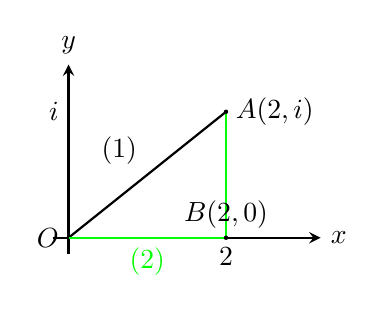
\begin{tikzpicture}[>=stealth,scale=1.0]
    % 坐标轴
    \draw[->,thick] (-0.2,0) -- (3.2,0) node[right] {$x$};
    \draw[->,thick] (0,-0.2) -- (0,2.2) node[above] {$y$};
    \node[left] at (0,0) {$O$};
    % 点 A(2,i) 与 B(2,0)
    \coordinate (A) at (2,1.6); % 这里用比例画出 i 的位置
    \coordinate (B) at (2,0);
    % 路径 (1)
    \draw[thick] (0,0) -- (A) node[midway,above left] {$(1)$};
    % 路径 (2)
    \draw[thick,green] (0,0) -- (B) node[midway,below] {$(2)$}
                      -- (A) node[midway,right] {};
    % 标记点与刻度
    \fill (A) circle (0.8pt) node[right] {$A(2,i)$};
    \fill (B) circle (0.8pt) node[above] {$B(2,0)$};
    \node[below] at (2,0) {$2$};
    \node[left] at (0,1.6) {$i$};
\end{tikzpicture}
\end{center}

\begin{solution}
先写出复函数的形式
\[
z^2 = x^2 - y^2 + i\,2xy.
\]

\textbf{路径 (1)：} 直线段 \(O\to A\)。

参数化取
\[
z(t)=(2+i)t,\qquad 0\le t\le 1,
\]
因此 \(dz=(2+i)\,dt\) 且
\[
z(t)^2=(2+i)^2 t^2=(3+4i)\,t^2.
\]
于是
\[
\int_{(1)} z^2\,dz
=\int_{0}^{1} (3+4i)t^2\,(2+i)\,dt
=(3+4i)(2+i)\int_{0}^{1} t^2\,dt.
\]
计算常数乘积与定积分：
\[
(3+4i)(2+i)=2+11i,\qquad \int_0^1 t^2\,dt=\frac{1}{3},
\]
因此
\[
\boxed{\;\int_{(1)} z^2\,dz=\frac{2}{3}+\frac{11}{3}i\;.}
\]

\bigskip

\textbf{路径 (2)：} 分两段，记为 (2a) 和 (2b)。

(2a) 实轴段 \(O\to B\)，参数化 \(z=x\) (\(0\le x\le 2\))，有 \(dz=dx\)，且 \(z^2=x^2\)。于是
\[
\int_{(2a)} z^2\,dz=\int_{0}^{2} x^2\,dx=\left.\frac{x^3}{3}\right|_{0}^{2}=\frac{8}{3}.
\]

(2b) 垂直段 \(B\to A\)，参数化 \(z=2+i y\) (\(0\le y\le 1\))，有 \(dz=i\,dy\)。计算
\[
z^2=(2+i y)^2=4- y^2 + i\,4y.
\]
因此
\[
\int_{(2b)} z^2\,dz
=\int_{0}^{1} (4- y^2 + i\,4y)\,i\,dy
=\int_{0}^{1}\big(4i - i y^2 -4y\big)\,dy.
\]
对每项积分得
\[
\int_0^1 4i\,dy = 4i,\quad
\int_0^1 (-i y^2)\,dy = -\frac{i}{3},\quad
\int_0^1 (-4y)\,dy = -2.
\]
故
\[
\int_{(2b)} z^2\,dz = -2 + \frac{11}{3}i.
\]

将两段相加得到路径 (2) 的总积分：
\[
\int_{(2)} z^2\,dz
= \frac{8}{3} + \Big(-2 + \frac{11}{3}i\Big)
= \frac{2}{3} + \frac{11}{3}i.
\]

\bigskip

两条路径的结果一致：
\[
\boxed{\;\int_{(1)} z^2\,dz=\int_{(2)} z^2\,dz=\frac{2}{3}+\frac{11}{3}i\;.}
\]
这符合期望，因为 \(f(z)=z^2\) 在全平面解析，因此对同一端点的曲线积分与路径无关（亦可由柯西定理/原函数原理说明：原函数为 \(F(z)=\tfrac{1}{3}z^3\)）。
\end{solution}




% \input{cauchy_theorem.tex}
% \input{cauchy_formula.tex}
% \section{复数级数}
% \input{series.tex}
% \input{convergence_test.tex}
% \input{power_series.tex}
% \input{taylor_laurent_series.tex}
% % \input{laurent_series.tex}
% \input{singular_points.tex}
% \section{留数定理及应用}
% \input{residue_theorem.tex}
% \input{residue_theorem_applications.tex}
% \input{feynman_technique.tex}
% \input{integral_demo.tex}

